
\documentclass[10pt,letterpaper]{article}

\usepackage{hyperref}
\usepackage{cogsci}
\usepackage[nodoi]{apacite}
\usepackage{pslatex}
\usepackage{pdfsync}
\usepackage{amsmath}
\usepackage{graphicx}
\usepackage{topcapt}
\usepackage{color}
\usepackage[english]{babel}
\usepackage{array}
\usepackage{pbox}



\title{Large-scale investigations of variability in children's first words}
\author{{\large \bf Rose M. Schneider} \\ \texttt{rschneid@stanford.edu}\\ Department of Psychology \\ Stanford University \\ 
\And {\large \bf Daniel Yurovsky} \\ \texttt{yurovsky@stanford.edu} \\ Department of Psychology \\ Stanford University \\ 
\And {\large \bf Michael C. Frank} \\ \texttt{mcfrank@stanford.edu} \\ Department of Psychology \\ Stanford University \\ }

\begin{document}
\maketitle


%ABSTRACT
\begin{abstract}
The first word, an intimate moment between child and caregiver, exhibits a tremendous amount of variability in semantic categorization, phonological complexity, and age of onset. Through several large datasets of parental report of children's first words, we investigate patterns in first word production. In three analyses, we explore the time course and distribution of children's first recognizable language productions. We find that, contra conventional wisdom, more than 75 percent of children in our datasets produce a first word by their first birthday. In our second analysis, we find that children consistently produce more first words in certain semantic categories. Finally, we take all the unique occurrences of words across the datasets, and try to predict first word production via parental input taken from the CHILDES corpus and the words' phonetic probabilities. Overall, we find that parental report of a child's first word yields rich and consistent data on what is typically an unobservable dyadic moment, and that consistencies in first word production across development may indicate a close relationship between conceptual and linguistic development.

\textbf{Keywords:}
language acquisition
\end{abstract}

%%INTRODUCTION%%%%
\section{Introduction}

The emergence of language in infancy is among the most astonishing developmental processes. Over the course of their first years, children rapidly go from speechless infants to toddlers producing and learning language at an astounding rate \cite{fenson1994,bloom2002}. Marking the beginning of productive verbal language, a child's first word is an important and measurable insight into what a child is willing and able to talk about at that point in their development. Yet, in contrast to later milestones, children's first words are an intimate moment between child and caregiver that is difficult for external observers to record or measure. Here we leverage large--scale data from parental reports to ask what children's first words reveal about two key issues in early language learning. 

First, from a very early point in development, infants exhibit an aptitude for language, even showing a preference for infant--directed over adult--directed speech at 1 month \cite{cooper1990}. Over the course of the first year, infants are learning to recognize the distinctive sounds and word forms of their native language \cite{kuhl2004} and to segment these phonetic forms and words \cite{werker2005}. Additionally, by 6 - 9 months, many infants already show a tendency to look to matching pictures when they hear common nouns, suggesting early beginnings for form-meaning mapping as well \cite{bergelson2012}. Infants' language comprehension abilities appear to be reasonably well-developed prior to 12 months. However, conventional wisdom holds that language production typically begins around the first birthday. Is this lag between comprehension and production real, or only apparent?

Second, what is the relationship between the words children learn and their conceptual development? Typically-developing monolingual children exhibit some particular relations between certain cognitive developments and language productions; for example, acquisition of words about disappearance is correlated with the comprehension of object permanence \cite{gopnik1986}. In contrast, 2 and 5 year--old international adoptees newly learning English show the same pattern of language acquisition as monolingual infants, both in time course and pattern of productive utterances \cite{snedeker2007}. This dissociation suggests that at older ages conceptual development may interact very little with word learning, but what about at younger ages with general referential language acquisition? Thus, when trying to untangle conceptual and linguistic development in infants, the first word is a very important as a measurable developmental milestone and as a more concrete indicator of a child's developmental state. Do patterns of first word productions suggest any relationship between language acquisition and cognitive development? 

Because very early language is difficult to observe in the lab, we leverage parent reports to learn about children's first words. A child's first word is highly memorable for parents, and many parents record this milestone in baby books. As a scientific measure, however, parent report has both drawbacks and advantages. One issue with any self--report measure is that there is no way to validate participants' responses. Another complication is that parents may be biased observers, and interpret word--like babble as productive communication. Parent report is widely used as a measure of early child language, e.g. in the MacArthur--Bates Communicative Development Inventory (CDI), a vocabulary checklist that is both a reliable and valid measure of early vocabulary \cite{fenson1994,fenson2007}. Nevertheless, the reliability of the earliest ages of the CDI has been questioned \cite{feldman2000}.

To address the issues of self--report, we gathered data from a number of sources. We specifically targeted different populations in our selections of data sources. The diversity of these four datasets encouraged a representative sample of children's first words, with each data source contributing its own set of advantages and drawbacks to the complete dataset. 

However, the data we received from these surveys was generally very consistent, both within and across datasets, indicating that parents responded appropriately. In addition to yielding reliable data, our first word surveys were highly effective, and were completed quickly and with minimal effort by many parents. 

Drawing on these datasets, we investigate the time course of the emergence of productive language and potential factors that might lead to individual differences in linguistic development. In Analysis 1, we investigate differences in age of first word onset, and find that 75 percent of children produce a word prior to 12 months. In Analysis 2, we explore whether early and later producers are sampling first words from conceptually different categories, and find no significant distribution in semantic categories before and after the first year. Finally, in Analysis 3, we turn to factors that may result in certain words and conceptual categories being more frequently produced as a first word ---- This will come later...

%%GENERAL DATA METHODS%%
\section{General Data Collection Methods}
Data for this study is comprised of four different datasets, each obtained from a different source. Three of the four datasets were drawn from surveys specifically designed for this study. The last dataset contains data from \href{http://wordbank.stanford.edu}{\tt{Wordbank}}, an online repository of data from the MacArthur--Bates Communicative Development Inventories (MB--CDI), a widely--used parent--report vocabulary checklist (Fenson et al., 2007).

The first dataset source, parents subscribed to The Children's Discovery Museum (CDM) mailing list, was chosen for collection because these parents were an ethnically diverse population with a higher education level than the general population, potentially leading to more accurate responses. For our next data source we targeted the Amazon Mechanical Turk (MTurk) population. This community is more representative of the general population in terms of age, gender, education level, and socio-economic status (SES). 

To complement our data from the general population, we next collected first word data from parents in the Psycholinguistic community (Info). This population was specifically selected for its familiarity with the subject as well as for highly accurate diary records. However, this population ended up being very small (N = 58).

Our final dataset, drawn from \href{http://wordbank.stanford.edu}{\tt{Wordbank}} was chosen because data points came from the MB-CDI, which is typically filled out closer in time to when the child produced her first word. A potential confound of the MB-CDI is a possible demand characteristic encouraging parents to report their children producing some word, as well as containing a somewhat limited set of potential words.

Overall, these methods of parental report yielded consistent and rich data with minimal time investment on behalf of the parent. However, as with most self--report measures, our surveys did have some disadvantages. While in every data collection we tried to stress that a first word was defined as a consistent set of sounds referring to the same referent across many contextual frames, we have no way of validating the parental report. Another issue was standardization of the child's first word, especially in the MTurk dataset, discussed below. 

%CDM
\subsection{Dataset 1: Children's Discovery Museum Survey}

\subsection{Participants}
We sent out a brief survey on children's first words to subscribed members of a large local children's museum. We received 502 responses to our survey (215 female, 285 male, and 2 with no reported sex; M age = 11 mo, median = 10 mo). Due to the diversity of the San Jose community, several of the first word responses were not in English. Responses were translated into English where possible. Responses that could not be translated were excluded from further analysis (N = 1). Guardian education level was not available for this population.

\subsection{Methods}
Parents completed a brief web--based survey (created with JavaScript and HTML). The survey asked parents to list their child's first word (excluding ``mama" and ``dada"), what they thought word referred to, a description of the situation surrounding the first word, the child's age at time of utterance (≤10 mo or younger, 11 mo, 12 mo, 13 mo, ≥14 mo), and the child's current age and sex. Parents answered for only one child in this survey.

\subsection{Data preparation}
Parents' responses were standardized for ease of analysis. Data cleaning involved fixing obvious spelling errors. When the meaning of the word was not immediately apparent, the researcher relied on the parent's description of the circumstances surrounding the word and/or the parent's classification of the word type.

%SURVEY2
\subsection{Dataset 2: Amazon Mechanical Turk}

\subsection{Participants}
We recruited 1000 parents from Amazon Mechanical Turk to complete an updated survey on their children's first words. We restricted the survey to parents in the United States. This survey allowed parents to answer for multiple children. We received 1671 responses (813 female, 858 male; M age = 10 mo, median = 10 mo). 21 children were excluded from subsequent analyses because they had not yet spoken (M age = 2.7 mo, median = 2 mo). Responses were translated into English when possible and required. Responses that were not able to be translated were excluded from further analysis (N = 1). Guardian education levels were highly diverse (Ns as follows: Elementary = 3; Some high school = 26; High school = 308; Some college = 525; College = 553; Some graduate school = 42; Graduate school = 26). 

\subsection{Methods}
This survey was an extended version of the previous one. The survey allowed for input for multiple children, and asked parents to list their highest education level, child's birth order, sex, first word (excluding ``mama" and ``dada"), word type, addressee of the first word, word age (0 - 24+ months), current age (0 - 18+ years), word language, and home language. Responses were validated as the survey was completed, reducing the likelihood of erroneous or false responses. 

\subsection{Data preparation}
Data were handled as in Dataset 1. Due to the larger sample size, more phonological and morphological variations appeared. A final standardized form was selected, and the various original first word forms became that standardized form. For example, ``Dog dog", ``Doggy", ``Doggie", and ``Dogie" were all treated as ``Dog" in the standardized form. We occasionally had to rely on the parent's description of the situation of the word occurrence to inform our decisions.

%%%SURVEY 3
\subsection{Dataset 3: Contemporary Psycholinguist Diary Studies}

\subsection{Participants}
We sent out a brief survey on children's first words to subscribed members of a Psycholinguist listserv. We received 52 responses from this survey (26 female, 26 male; M age = 11.16 mo, median 11 mo).

\subsection{Methods}
Questions included on the survey were: The approximate phonological form of the first word, the age of the utterance, when the parent recorded this (if at all), the child's sex, the target word, the child's birth order (first or later born), and the child's current age. 

\subsection{Data processing}
Data were handled similarly to Datasets 1 and 2. 

%%%%WORDBANK%%%%
\subsection{Dataset 4: MB--CDI Wordbank}

\subsection{Participants}
At the time of our analysis, the Wordbank database contained 949 unique MCDI Words and Gestures administrations. From these, we selected the 76 children whose parents reported that they produced exactly one word (31 female, 45 male, M age = 10.63 mo, median = 11 mo). Guardian education levels were fairly diverse (Ns as follows: Some high school = 4; High school = 24; Some college = 21; College = 17; Some graduate school = 1; Graduate school = 9). 

\subsection{Data preparation}
Because responses were taken directly from parental reports on the MB-CDI, no data preparation was necessary.

%Analyses
\section{Analyses}
The emergence of language in infancy has long been the focus of research and discussion. Noun comprehension has been shown to occur prior to production, indicating a conceptual understanding of label-referent mapping at 6-9 months \cite{tincoff1999,tincoff2012,bergelson2012}. As early as 12 weeks, children begin producing the sounds of their native language /cite{kuhl1996}, suggesting an early beginning to linguistic development. Yet the first word is not typically expected until around 12 months. Does a lag between comprehension and production exist, and what is the relationship between the words that children learn and their conceptual development? 

In analyzing this data, we are interested first in understanding the timeline of the emergence of productive language and the factors predicting this emergence in individuals. We explore whether productive language lags comprehension with an analysis of children's ages at the time of their first words. We find that 75\% of children produce a first word by 12 months as well as evidence of a wide age range in which the first word is typically uttered.

We next turn to the question of why some children are producing language earlier than others, and if this reveals anything about the relationship between conceptual and linguistic development. First, we compare distributions of semantic (CDI) categories in first word productions in children older and younger than 12 months. If early producers' CDI category distributions are significantly different than later producers', this could indicate a loose coupling of linguistic and conceptual development. However, we find that both before and after the first year, children's first words tend to come from the same conceptual categories.

We do not find that later producers are sampling words from a different or more diverse range of conceptual categories, but instead find that children across development are speaking about the same kinds of things, and often even the same things. What makes these words more likely to be produced as a first word, if they do not significantly differ conceptually? In our final analysis, we examined both the phonetic probability of individual words within CDI categories, as well as their correlation with parental input in an attempt to determine why some words are consistently produced before others. The results of this analysis indicate that fewer phonemes and increased input frequency within CDI categories predict first words production.

Overall, we find that if a lag between comprehension and general referential production exists in development, it is much shorter than previously thought, and most likely driven by developing linguistic capacities and not by a cognitive shift. Furthermore, our results suggest that conceptual and linguistic development are closely linked, and although the age of onset for productive language may vary across children, the semantic referents of first words are likely to be fairly consistent. Finally, we suggest that first words within semantic categories are predicted by phonetic complexity and input frequency. 

\subsection{Exclusion of ``mama'' and ``dada''}
While many parents reported that their child's first word was ``mama'' or ``dada'' (or some variant), we excluded these children from our analyses. Parents may be motivated to hear these words very early in babble, even when the word is not being used in a meaningful or consistent way. Therefore, we stressed in our surveys that parents were to report their children's first word $other$ than ``mama'' or ``dada'' to avoid the possibility of skewing the data. After pilot testing on Amazon Mechanical Turk, we added another question asking whether the child's first utterance was ``mama'', ``dada'', or another first word. 1112 parents reported their children producing ``mama'' (N = 618) or "dada" (N = 494) rather than another word (N = 559) as a first utterance. 

\subsection{Age} 

Despite evidence for very early word comprehension \cite{tincoff1999,tincoff2012,bergelson2012}, conventional wisdom generally holds that first word emerges at around 12 months. However, a child's first word is almost exclusively heard by a parent or other caretaker and can be very difficult for an external observer to measure. Is this reported lag between comprehension and production real or apparent?  Given the possibility of very early noun comprehension \cite{tincoff1999,tincoff2012,bergelson2012}, we wished to explore the development of first word production, especially prior to 12 months.

Across the 4 datasets, we grouped data by age and by dataset, $N_{total} = 3173$. Twenty--one children were excluded for not having spoken yet (M age = 2.7 mo, median = 2 mo). We then plotted the cumulative probability of a child having produced a first word as a function of their age (Figure 1).

%FIGURE 1
\begin{figure}[t]
\center{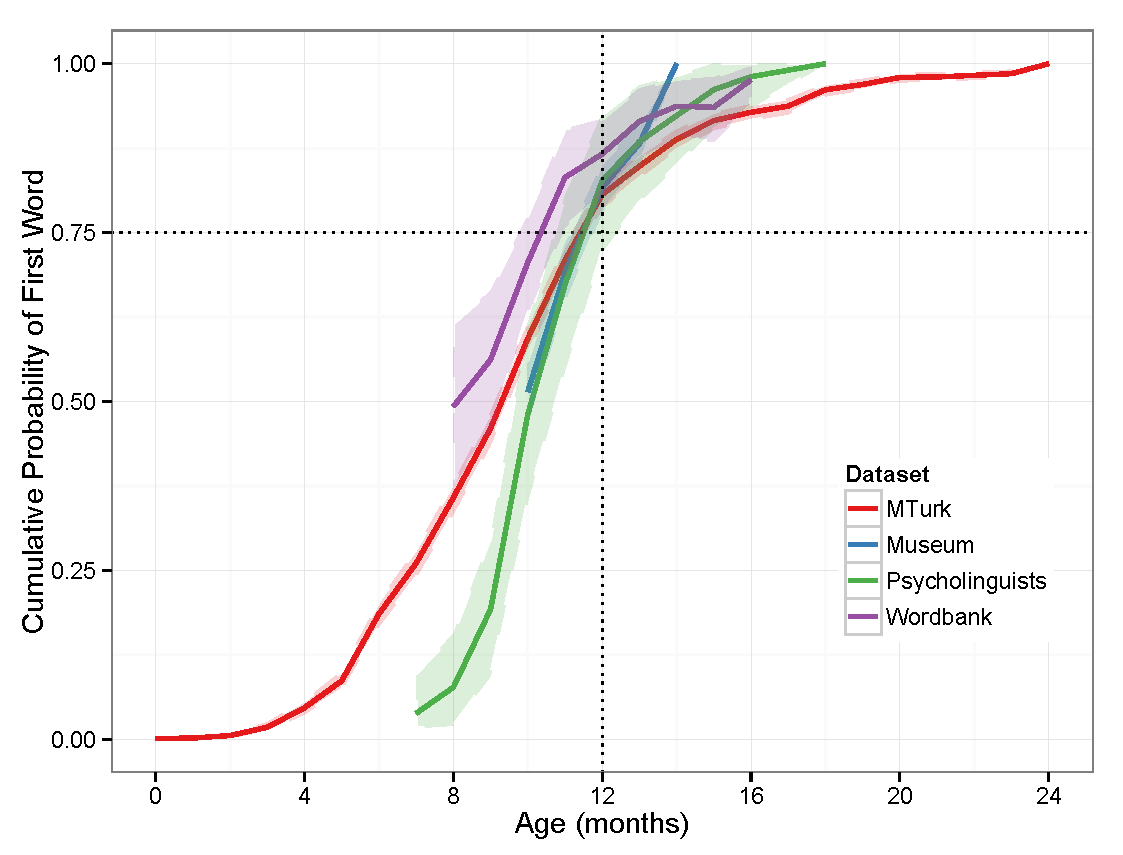
\includegraphics[width=.48\textwidth]{figures/agedata_4sets.pdf}}
\caption{\label{fig:cdfs} Age graph showing the cumulative probability of producing a word as a function of age.}
\end{figure}

Prior to 12 months, approximately 75\% of children have produced a first word, and we see a gradual but consistent increase from 12--24 months. The plot of the Mechanical Turk data, the largest dataset, is most likely the most representative of child word production, while the other datasets asymptote fairly quickly between about 14 and 17 months. These data suggest that production may not lag comprehension as much as previously thought. To discern whether there might be a bias on behalf of parents of older children to report a younger first word, we ran a (TEST), but did not receive a significant result ($p > XX$).


\subsection{CDI Categories} 
Why are some children producing language earlier than other children, and what does this reveal about the relationship between their conceptual and linguistic development? Previous work has established that the CDI normative categories are not equally represented in first word production \cite{fenson1994}. When children produce early language ($<$12 months), are they choosing to produce conceptually different words than children who speak later? Or, are conceptual and linguistic development more closely linked, with the same semantic categories appearing as first words regardless of age of utterance? In our next analysis, we examined the CDI category frequencies of children's first words to explore whether very early first words differ conceptually from later--produced words. 

In this analysis, CDI categories were assigned by the researcher based on the MB--CDI parental report form, and validated across datasets. In instances where words did not appear on the MB--CDI, categories were assigned ad hoc and validated across datasets for consistency. Ninety--one children were excluded because their first word was unable to categorized. We grouped the data by dataset, and performed an age split at 12 months. Figure 2 shows the frequencies of the CDI categories split by age and grouped by dataset.

%FIGURE 2
\begin{figure}[tb]
\center{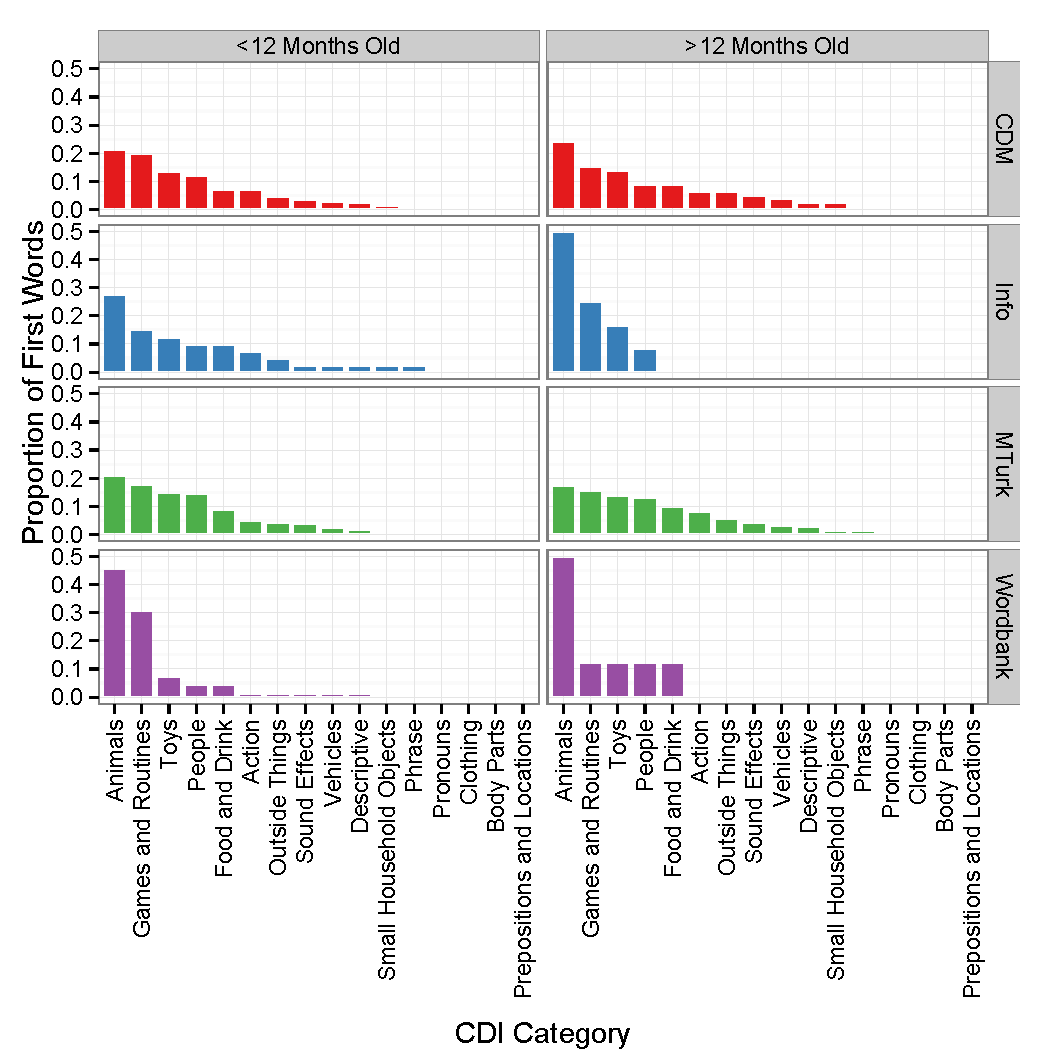
\includegraphics[width=.45\textwidth]{figures/cdicats_4sets.pdf}}
\caption{\label{fig:cdfs} Histogram of CDI category frequencies across datasets.}
\end{figure}

Distributions of CDI category frequency across all 4 datasets were quite similar. We constructed a linear model, and did not find an effect of dataset on CDI category distribution ($p > XX$). Although more children are included in the $>$ 12 month group, the distributions of the CDI category representations remain very similar.

Animals, Games and Routines, Toys, and People, followed closely by Food and Drink are frequent first word categories, and seem to be equally compelling as a first word for both early and later producers. Data for later speakers in Wordbank is sparse, because children were selected for this analysis when they were producing exactly one word, according to parental report on the MB--CDI. Only 27 children produced only exactly word in this group.

Despite producing a first word during different points in their conceptual development, both early and later producers are choosing to speak about the same semantic categories, and in many cases, the same things (Figure 3). This would suggest that children's linguistic and conceptual development are more intimately related, and the production of a first word is possibly not the result of a cognitive shift, but an ability to produce and form words.


%FIGURE 3

\begin{table}[t]
\centering
\begin{tabular}{cccc}
\hline
{\bf CDM} & {\bf MTurk} & {\bf Info} & {\bf Wordbank} \\ 
\hline
Ball & Dog & Up & Baa Baa \\ 
Hi & No & More & Uh--Oh \\
Dog & Ball & Hi & Yum Yum \\ 
Uh--Oh & Bottle & Cat & Woof Woof \\ 
Duck & Hi & Bye & Hi \\ 
\hline 
\end{tabular}
\caption{\label{tab:top5} Top 5 first words (excluding ``mama'' and ``dada'') from each of the four datasets we examined.}
\end{table}

However, out of all the sets of possible first words, why are children consistently choosing to produce words predominantly from these semantic categories? What is tipping the balance in favor of these particular words? Some potential factors are frequency of parental input, the phonetic probability and ease of production. In the next analysis, we examine all of these within CDI categories to attempt to untangle what causes the measure of consistency we observe in first word productions.


\section{Predicting First Words}

Our previous analyses found a high degree of consistency among children's first productions. Independent of age, gender, and birth order, children seem to produce the same first words. Why these words? To say a word, a child must minimally have been exposed to that word, and also be able to pronounce it. We thus consider two factors known to predict the acquisition of words more broadly: input frequency, and phonetic complexity \cite{goodman2008}.

\subsection{Method}

Because the set of all possible words is infinite, it is impossible to normalize correctly. Thus, we chose to use a representative set that would allow us to have the same basis for comparison across datasets: the 385 words on the MB-CDI Words and Gestures form. We thus chose the subset of words in each of our datasets that appeared on the CDI, and asked about the relative probability of production of each of these words.

To estimate the frequency with children hear each of these words, we counted the number of times each appeared in CHILDES---a large corpus of parent-child interactions \cite{macwhinney2000}. In order to ensure a representative sample, we counted the number of appearances of each word in a child's mother's speech across all of the corpora in the North American subset of CHILDES. These frequencies were then log-transformed and used to predict first words.

To estimate phonetic complexity, we chose a simple, theory-independent measure: number of phonemes. For each of this same subset of words, we queried the MRC Psycholinguistic Database \cite{Wilson1988}. Number of phonemes is an imperfect measure of phonetic complexity---e.g. it misses differences in articulatory complexity that contribute to the relative difficulty of producing different words (e.g. ``truck'' vs. ``bunny'')---but it does capture much of the variability among the CDI words.

To predict the effects of continuous predictors on count outcomes, it is common to use Poisson regression. However, Poisson regression behaves poorly in practice because empirical counts violate its assumptions in two ways: their variance is greater than expected (over dispersion), and too many of them are zero (zero inflation). To adjust for these violations, we used a hurdle model that adds a second component to Poisson regression: a binomial threshold (hurdle) that first determines whether a count is-nonzero \cite{mullahy1986}. Because the datasets were of such different sizes, we fit a separate hurdle regression to each.

\subsection{Results and Discussion}

Across datasets, input frequency and phonetic complexity consistently predicted the number of children who produced each word as their first word. As we predicted, in almost all cases words were more likely to be produced as a child's first word if they were higher frequency in children's input, and had few phonemes (Figure~\ref{fig:hurdles}). In conjunction with the analyses above, these results suggest a high degree of consistency in children's first productions, independent of demographic factors and conceptual development, and dependent instead on linguistic input and speech production fluency.

(ASIDE: Wordbook goes the other way, check against the understood words).

\begin{figure}[tb]
\center{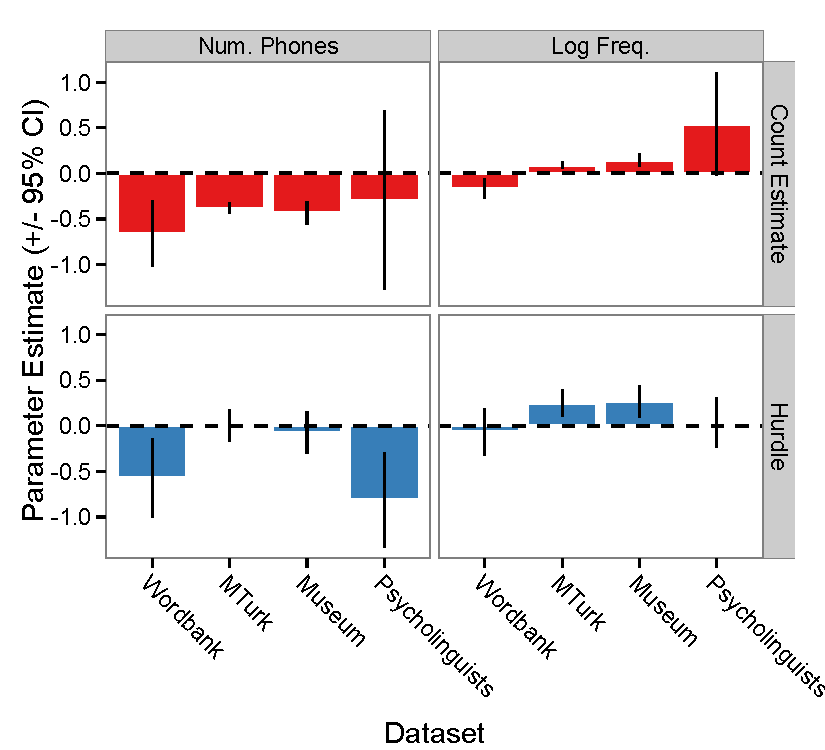
\includegraphics[width=.48\textwidth]{figures/hurdle_params.pdf}}
\caption{\label{fig:hurdles} Parameter estimates for hurdle models predicting children's first words. Models showed a high degree of consistency across datasets: first words tend to be higher frequency and have fewer phonemes. Intercepts are omitted for clarity.}
\end{figure}

\section{Discussion}

\section{Acknowledgements}


\bibliographystyle{apacite}

\setlength{\bibleftmargin}{.125in}
\setlength{\bibindent}{--\bibleftmargin}

\bibliography{fw_cogsci}

\end{document}


